\documentclass[12pt,letterpaper]{article}
\usepackage{fullpage}
\usepackage[top=2cm, bottom=4.5cm, left=2.5cm, right=2.5cm]{geometry}
\usepackage{amsmath,amsthm,amsfonts,amssymb,amscd}
% \usepackage{lastpage}
\usepackage{enumerate}
\usepackage{fancyhdr}
% \usepackage{mathrsfs}
\usepackage{xcolor}
\usepackage{graphicx}
\usepackage{listings}
\usepackage{hyperref}

\usepackage{float}

% define vector
\newcommand{\q}{\underline}
\newcommand{\mt}{\mathrm}

\setlength{\parindent}{0.2in}
\setlength{\parskip}{0.1in}

% Edit these as appropriate
\newcommand\course{Phys 213}
\newcommand\hwnumber{4}                  % <-- homework number
\newcommand\Name{M.-F. Ho}

\pagestyle{fancyplain}
\headheight 35pt
\lhead{\Name}
\chead{\textbf{\Large Homework 4}}
\rhead{\course \\ \today}
\lfoot{}
\cfoot{}
\rfoot{\small\thepage}
\headsep 1.5em

\newcommand{\Data}{\mathcal{D}}
\newcommand{\xvec}{\boldsymbol{x}}
\newcommand{\Xvec}{\boldsymbol{X}}
\newcommand{\Var}{\textrm{Var}}
\newcommand{\normal}{\textrm{N}}
\newcommand{\uniform}{\textrm{U}}
\newcommand{\xmean}{\langle \xvec \rangle}
\newcommand{\newx}{\tilde{x}}
\newcommand{\integer}{\mathbb{N}}
\newcommand{\thetarv}{\tilde{\theta}}
\newcommand{\phirv}{\tilde{\phi}}

\newcommand{\ml}{m_{\ell}}
\newcommand{\specterms}{^{2S+1}\mathcal{L}^p_\mathcal{J}}
\newcommand{\EWrest}{W^{\mt rest}_\lambda}
\newcommand{\lambdarest}{\lambda_{\textrm{rest}}}

\newcommand{\FeII}{\textrm{Fe\,II}}
\newcommand{\CII}{\textrm{C\,II}}
\newcommand{\columndensity}{N_\ell}
\newcommand{\columndensityrv}{\tilde{\columndensity}}
\newcommand{\kms}{\textrm{\,km/s}}
\newcommand{\dvfwhm}{(\Delta v)_{\textrm{FWHM}}}

\begin{document}

\section*{1 (a): C.O.G}

The approximated equation listed in Draine is:
\begin{equation}
    W \simeq \sqrt{\pi} \frac{b}{c} 
    \frac{\tau_0 }{1 + \tau_0 / (2\sqrt{2})},
\end{equation}
for $\tau_0 < 1.25393$.
And:
\begin{equation}
    W \simeq
    \sqrt{ 
        (\frac{2b}{c})^2 \ln{\frac{\tau_0}{\ln{2}}} +
        \frac{b}{c} \frac{\gamma_{\ell e}\lambda_{\ell u}}{c}
        \frac{(\tau_0 - 1.25393)}{\sqrt{2}}
     },
\end{equation}
for $\tau_0 > 1.25393$.

The question nastily only gives us $W^{\mt rest}_\lambda$ with a unit,
so we have to convert it to the dimensionless $W$.
The conversion should be given in eq (9.4) in Draine:
\begin{equation*}
    W_\lambda = \int d\lambda (1 - e^{-\tau_\nu}) \simeq \lambda_0 W,
\end{equation*}
so ideally we have $W \simeq W_\lambda / \lambda_0$.

\begin{itemize}
    \item Fe II: $W \simeq \EWrest / \lambdarest = 0.051 / 2382.7642 = 2.140 \times 10^{-5}$
    \item Fe II: $W \simeq \EWrest / \lambdarest =  0.0047 / 2249.8768 = 2.089 \times 10^{-6}$
    \item C II:  $W \simeq \EWrest / \lambdarest =  0.060 / 1334.5323 = 4.496 \times 10^{-5}$
\end{itemize}

Now the strategy is to determine which equation to use.
Since we consider ranges $\log{N_{\FeII}} \sim \uniform(12, 16)$ and $\log{N_{\CII}} \sim \uniform(13, 17)$.
Consider the definition of $\tau_0$ as function of $N_\ell$:
\begin{equation}
    \begin{split}
        \tau_{0, \columndensityrv}(\columndensity)
        &= \sqrt{\pi}\frac{e^2}{m_e c} \columndensity
        f_{\ell u} \lambda_{\ell u} \frac{1}{b}(1 - \frac{N_u / g_u}{N_\ell / g_\ell})\\
        &= 1.497 \times 10^{-2} \frac{\mt{cm}^2}{s} \frac{f_{u \ell}\lambda_{\ell u}}{b} N_\ell,
    \end{split}
    \label{eq:tau_0}
\end{equation}

After plugging the numbers into eq~\ref{eq:tau_0}, unfortunately the values of $\tau_0$ is not falling just one-side of the $\tau_0 = 1.25393$:
\begin{equation*}
    \tau_{0,\columndensityrv}(\columndensity, b=10, f=0.320, \lambdarest=2382.7642)
    = (0.11, 1141.44).
\end{equation*}
We thus have to consider both equations.

We clearly know the form of $\tau_0$, so it's a matter of making decisions for plotting.
The way I implemented is estimating $\tau_0$ first based on given $b$ and $\columndensity$, and using the value of $\tau_0$ to determine which equation we are going to use to compute $W$. 
Finally, convert $W$ to $W_{\lambda}$ using $\lambda_0 W$.

Here are examples of dimensionless W C.O.G:
% plotting C.O.G for W
\begin{figure}[H]
    \centering
    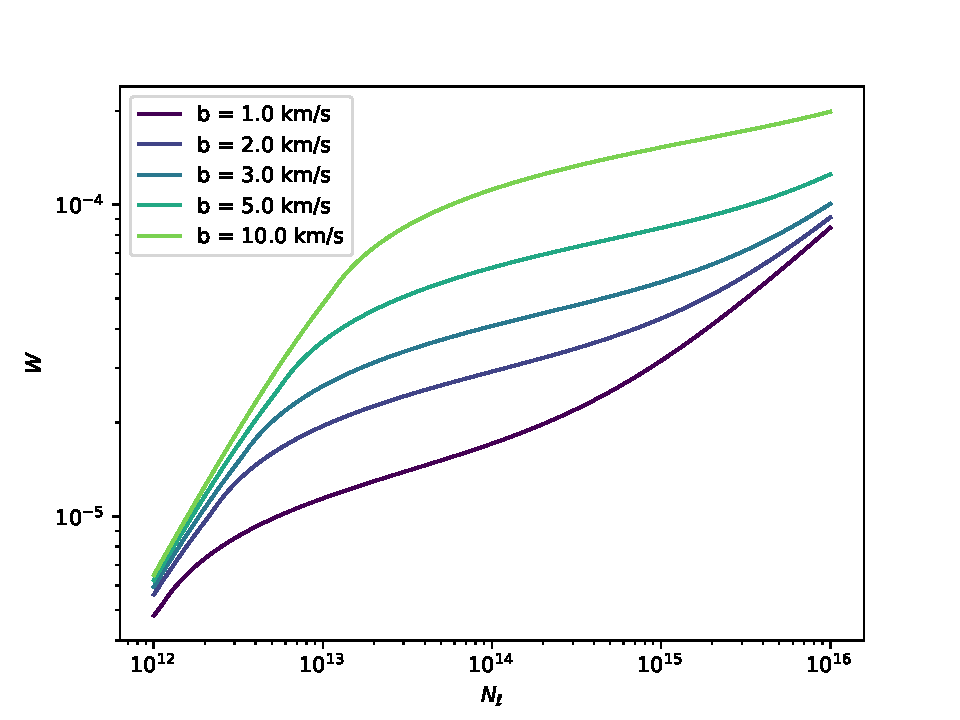
\includegraphics[width=0.75\columnwidth]{images/W_N_Fe_II_1.pdf}
    \caption{Fe II, $\lambdarest = 2382.7642$ \AA}
\end{figure}
\begin{figure}[H]
    \centering
    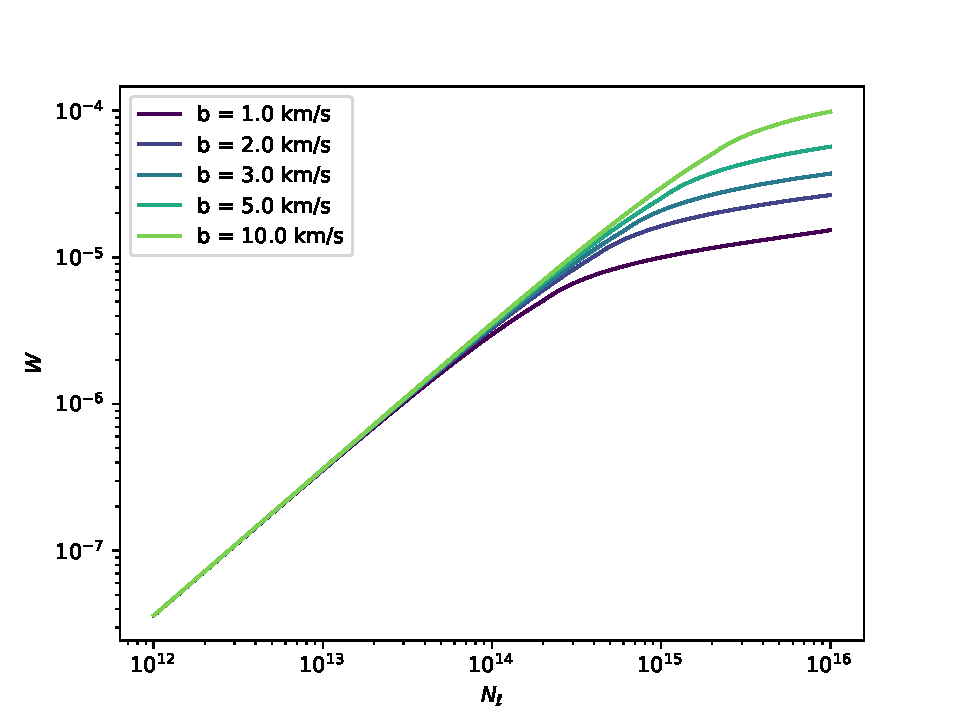
\includegraphics[width=0.75\columnwidth]{images/W_N_Fe_II_2.pdf}
    \caption{Fe II, $\lambdarest = 2249.8768$ \AA}
\end{figure}
\begin{figure}[H]
    \centering
    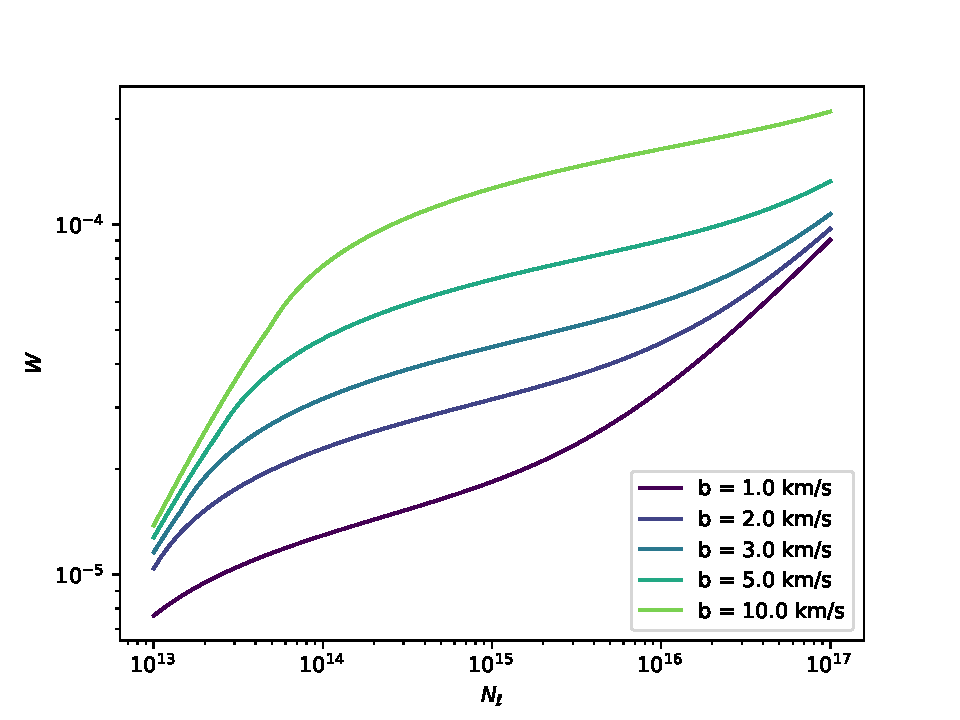
\includegraphics[width=0.75\columnwidth]{images/W_N_C_II.pdf}
    \caption{C II, $\lambdarest = 1134.5323$ \AA}
\end{figure}

Here are examples of $\EWrest$ C.O.G:
% plotting C.O.G for W
\begin{figure}[H]
    \centering
    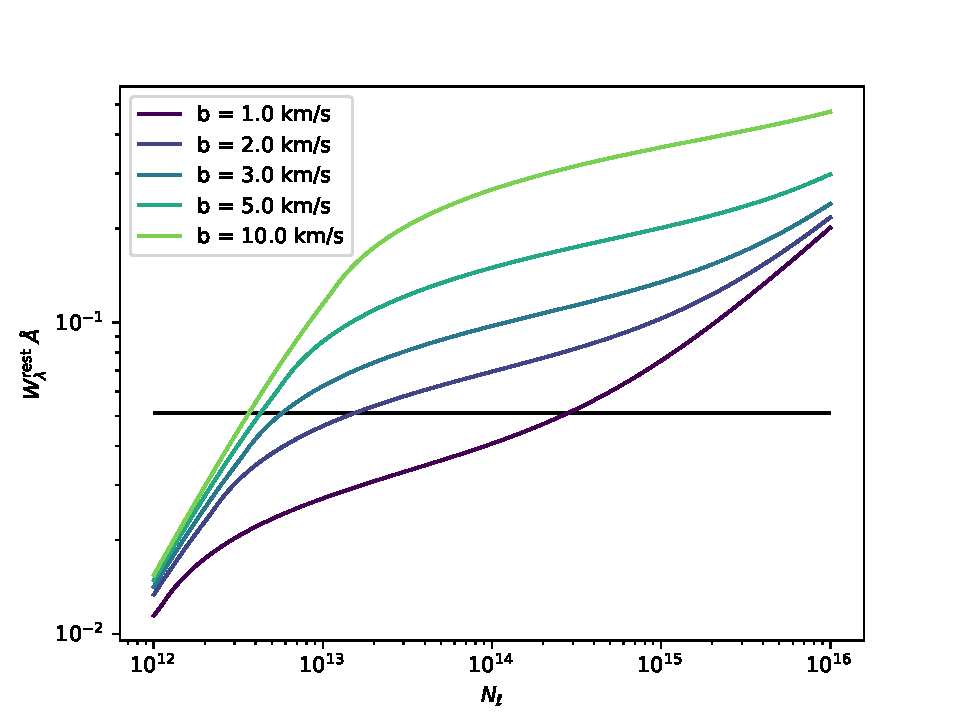
\includegraphics[width=0.75\columnwidth]{images/Wl_N_Fe_II_1.pdf}
    \caption{Fe II, $\lambdarest = 2382.7642$ \AA}
    \label{fig:Fe_II_2382}
\end{figure}
\begin{figure}[H]
    \centering
    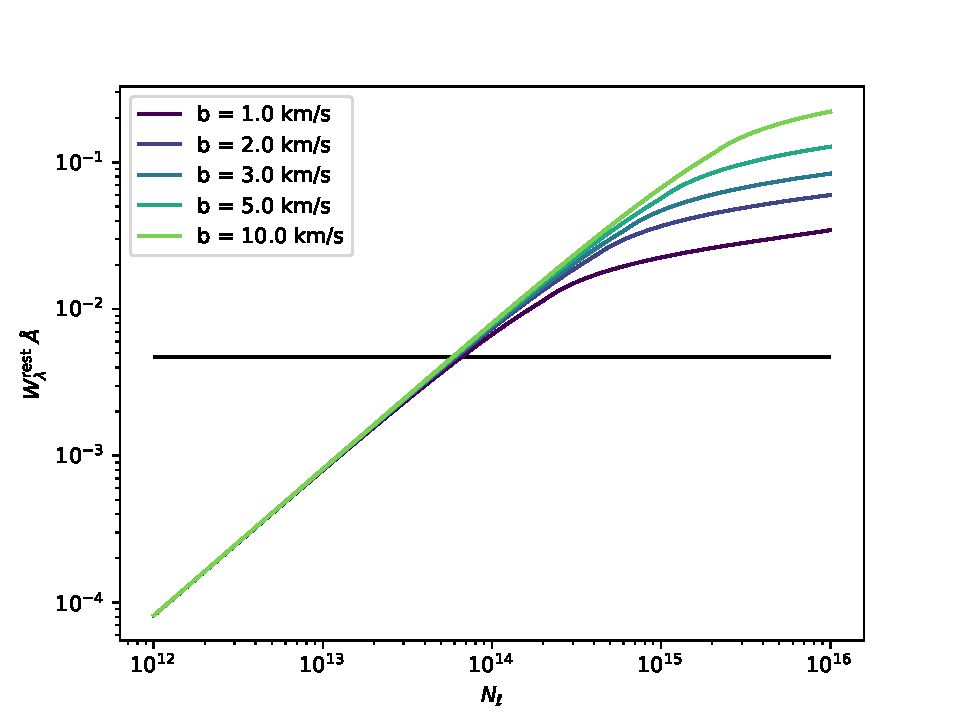
\includegraphics[width=0.75\columnwidth]{images/Wl_N_Fe_II_2.pdf}
    \caption{Fe II, $\lambdarest = 2249.8768$ \AA}
    \label{fig:Fe_II_2249}
\end{figure}
\begin{figure}[H]
    \centering
    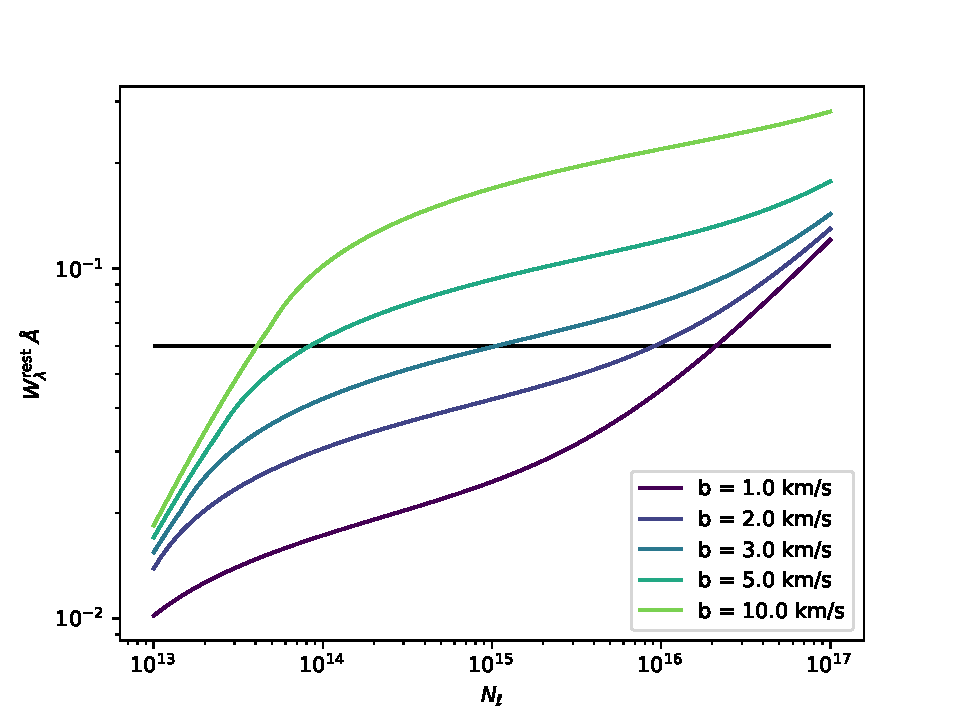
\includegraphics[width=0.75\columnwidth]{images/Wl_N_C_II.pdf}
    \caption{C II, $\lambdarest = 1134.5323$ \AA}
    \label{fig:CII}
\end{figure}

The black lines I plotted there are the observed $\EWrest$ of these lines.
Previously (in the previous version), I set a wrong $c=10^{11} cm/s$, which should be corrected as $c = 10^{10} cm/s$.
Here the black lines are nicely crossing the COG.

\section*{1 (b): Fe II Metallicity}
The question asks us to identify the value of b parameters based on the plots we plotted in the question (a).
We probably could solve it analytically, but I think the question asked us to find the value by eyes.

Based on the curves, we see only Fig~\ref{fig:Fe_II_2249} has a stable solution for $N_\ell$, which gives $N_\ell \simeq 10^{13.6} cm^{-2}$.
This column density could be used to solve the $b$ for FeII with $2382.7642$ \AA.
The argument is both FeII lines should have the same $N_\ell$.
By squinting Fig~\ref{fig:Fe_II_2382}, we roughly get $b\sim1.5\kms$.

Now it's the matter of converting $b$ to $\dvfwhm$.
With the help from Draine:
\begin{equation}
    \dvfwhm = 2 \sqrt{\ln{2}}\, b.
\end{equation}
You can think this is the property of a normal distribution, that the FWHM has a nice relation with the standard deviation.
For this particular line FeII $2382.7642$ \AA, :
\begin{equation*}
    \dvfwhm = 2 \sqrt{\ln 2} \, 1.5 \kms \simeq 2.5\kms,
\end{equation*}

The thing is we should expect the velocity being stretched by the redshifting of the universe by a factor of $(1 + z)$:
\begin{equation}
        \dvfwhm^{obs}  = (1+z) \times 17 \simeq 7.5 \kms
\end{equation}

The thing is the resolution of HIRES is around $7-9 \kms$.
So it's hard to tell wether it is resolvable or not.

We now are supposed to calculate the metallicity:
\begin{equation}
    [Fe/N] = \log{(N_{Fe} / N_H}) - \log{(N_{Fe} / N_H)}_\odot.
\end{equation}
Now we steal the table from  Asplund et al. 2009,
ARAA, 47, 481, which is suggested by the instructor:
\begin{figure}[H]
    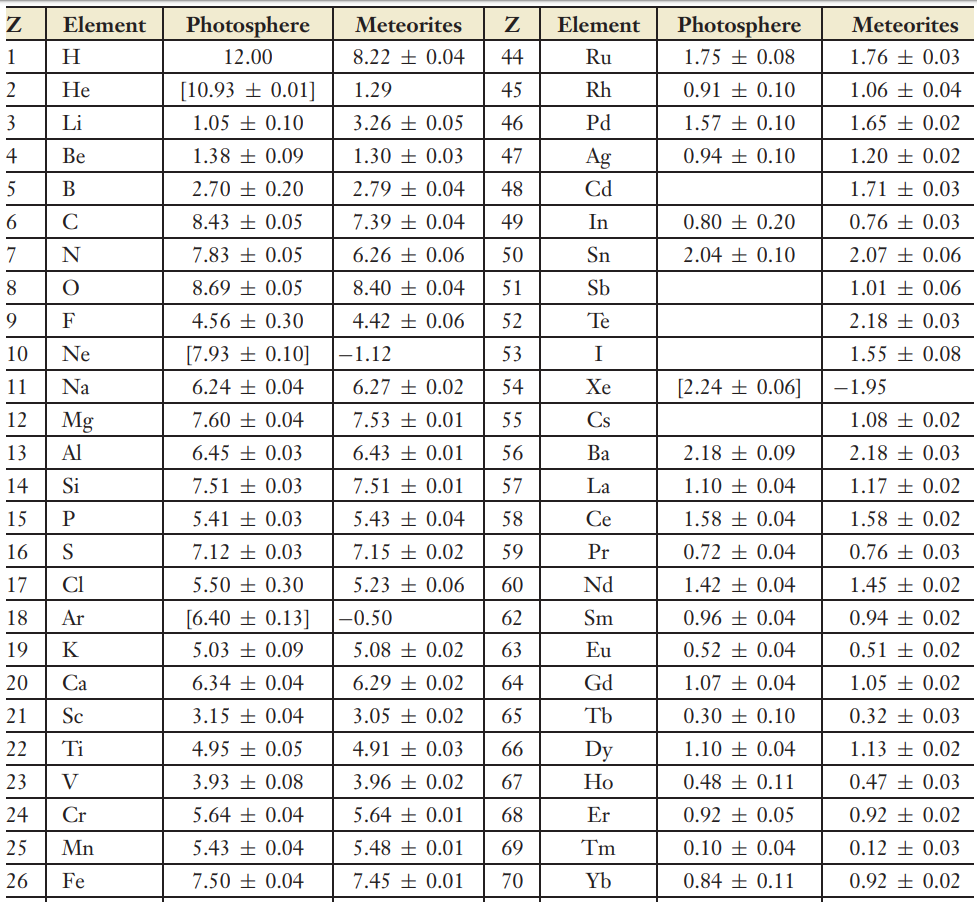
\includegraphics[width=\columnwidth]{images/photosphere.png}
\end{figure}
To compute the solar metallicity, we grab the photosphere values from H and Fe:
\begin{equation*}
    \log{(N_{Fe} / N_H)}_\odot = 7.5 - 12 = -4.5
\end{equation*}
Thus,
\begin{equation*}
    [Fe/H] = 
    \log{(N_{Fe} / N_H)} - \log{(N_{Fe} / N_H)}_\odot =
    \log{(10^{13.6} / 10^{20.3})} - (-4.5) = 
    13.6 - 20.3 + 4.5 = -2.2.
\end{equation*}

\section*{1 (c): CII Metallicity}
I did not know this before I read the solution.
But for turbulent broadening, all ions of the system have the same $b$s.
So CII will have $b \sim 1.5\kms$, the same as FeII $2382$ \AA in the previous question.

By squinting the Fig~\ref{fig:CII}, we roughly get $N_\ell \sim 10^{16.5} cm^{-2}$.

Now we carry out the metallicity:
\begin{equation*}
    \begin{split}
        [C\,II/H] &= 
        \log{(N_{CII} / N_H)} - \log{(N_{CII} / N_H)}_\odot =\\
        &= \log{(10^{16.5} / 10^{20.3})} - ( 8.43 - 12 ) \approx 
        16.5 - 20.3 + 3.57 = -0.23.                
    \end{split}
\end{equation*}

Comparing to FeII,
\begin{equation*}
    [C\,II, Fe\,II] = \log{(N_{CII} / N_{FeII})} - \log{(N_{CII} / N_{FeII})}_{\odot}
    = 16.5 - 13.6 - (8.43 - 7.5) = 1.97.
\end{equation*}


\section*{1 (d): Thermally broadening}
We know the thermal velocity is also a Gaussian like distribution, so the FWHM could be written as:
\begin{equation}
    \dvfwhm^{\textrm{thermal}} = 2 \sqrt{\ln 2} \left( \frac{k T}{M} \right)^{1/2} 
    = 2.15 \left( \frac{T / 100\, \mt K}{M / m_H} \right)^{1/2} 
    \kms,
    \label{eq:thermal}
\end{equation}
where we know $M_{Fe} / m_H \simeq 56$.
We would thus be able to infer the value of T if we assume thermal velocity contribute to the $b$ we observe from the plots.

The least condition for these lines being dominated by thermal broadening is that the $\dvfwhm^{\textrm{thermal}} > \dvfwhm$.
\begin{equation*}
    \begin{split}
        &\dvfwhm^{\textrm{thermal}} > \dvfwhm\\
        &\Rightarrow
        2.15 \left( \frac{T / 100\, \mt K}{M / m_H} \right)^{1/2} 
    \kms >  \dvfwhm\\
        &\Rightarrow
        T / 100\, {\mt K} > 1/(2.15)^2 * \frac{M}{m_H} \dvfwhm^2\\
        &\Rightarrow 
        T > 100/2.15^2 * 56 * 2.5^2 K \simeq 7571.7\,K
    \end{split}
\end{equation*}


\section*{1(e) Infer b for thermal broadening}
Since we have Eq~\ref{eq:thermal}, we thus know $\dvfwhm^{\textrm{thermal}} \propto \frac{1}{\sqrt{M_X}}$, where $X \in \{\textrm{ions}\}$.
By the linear relationship between $\dvfwhm^{\textrm{thermal}}$ and $b$, we have:
\begin{equation*}
    b \propto \frac{1}{\sqrt{M_X}},
\end{equation*}
where $X \in \{\textrm{ions}\}$.
Thus $b$ for CII is estimated by $\sqrt{\frac{M_{FeII}}{M_{CII}}} b_{FeII} = 5.4 \kms$.
The corresponding $N_\ell$ would be $N_\ell = 10^{12.3} cm^{-2}$ by squinting.

The value of metallicity would be:
\begin{equation*}
    \begin{split}
        [C\,II/H] &= 
        \log{(N_{CII} / N_H)} - \log{(N_{CII} / N_H)}_\odot =\\
        &= \log{(10^{12.3} / 10^{20.3})} - ( 8.43 - 12 ) \approx 
        12.3 - 20.3 + 3.57 = -4.43.                
    \end{split}
\end{equation*}

Comparing to iron:
\begin{equation*}
    [C\,II, Fe\,II] = \log{(N_{CII} / N_{FeII})} - \log{(N_{CII} / N_{FeII})}_{\odot}
    = 12.3 - 13.6 - (8.43 - 7.5) = -2.29.
\end{equation*}


\section*{1 (f): Carbon enhanced}
Given that carbon rich DLA is rare, it's more possible that thermal broadening is the dominated effect since it gives lower carbon abundance.


\end{document}
